\begin{titlepage}
	\begin{tikzpicture}[remember picture,overlay]
	%% Heading
	\node[text width=1.0\textwidth] at ($$ (current page.north) + (0mm,-70mm) $$){
		\begin{center}
			{\Huge\sffamily\textbf{\textit{OpenLB User Guide}}}\\[0.5cm]
			{\Large\sffamily\textbf{\textit{Associated with Release 1.9 of the Code}}}
        \end{center}
	};
	%% Title-image
		\node[text width=1.0\textwidth] at ($$ (current page.center) + (0mm,15mm) $$){
		\begin{center}
		%\includegraphics[width=11cm]{fig/face.png}
		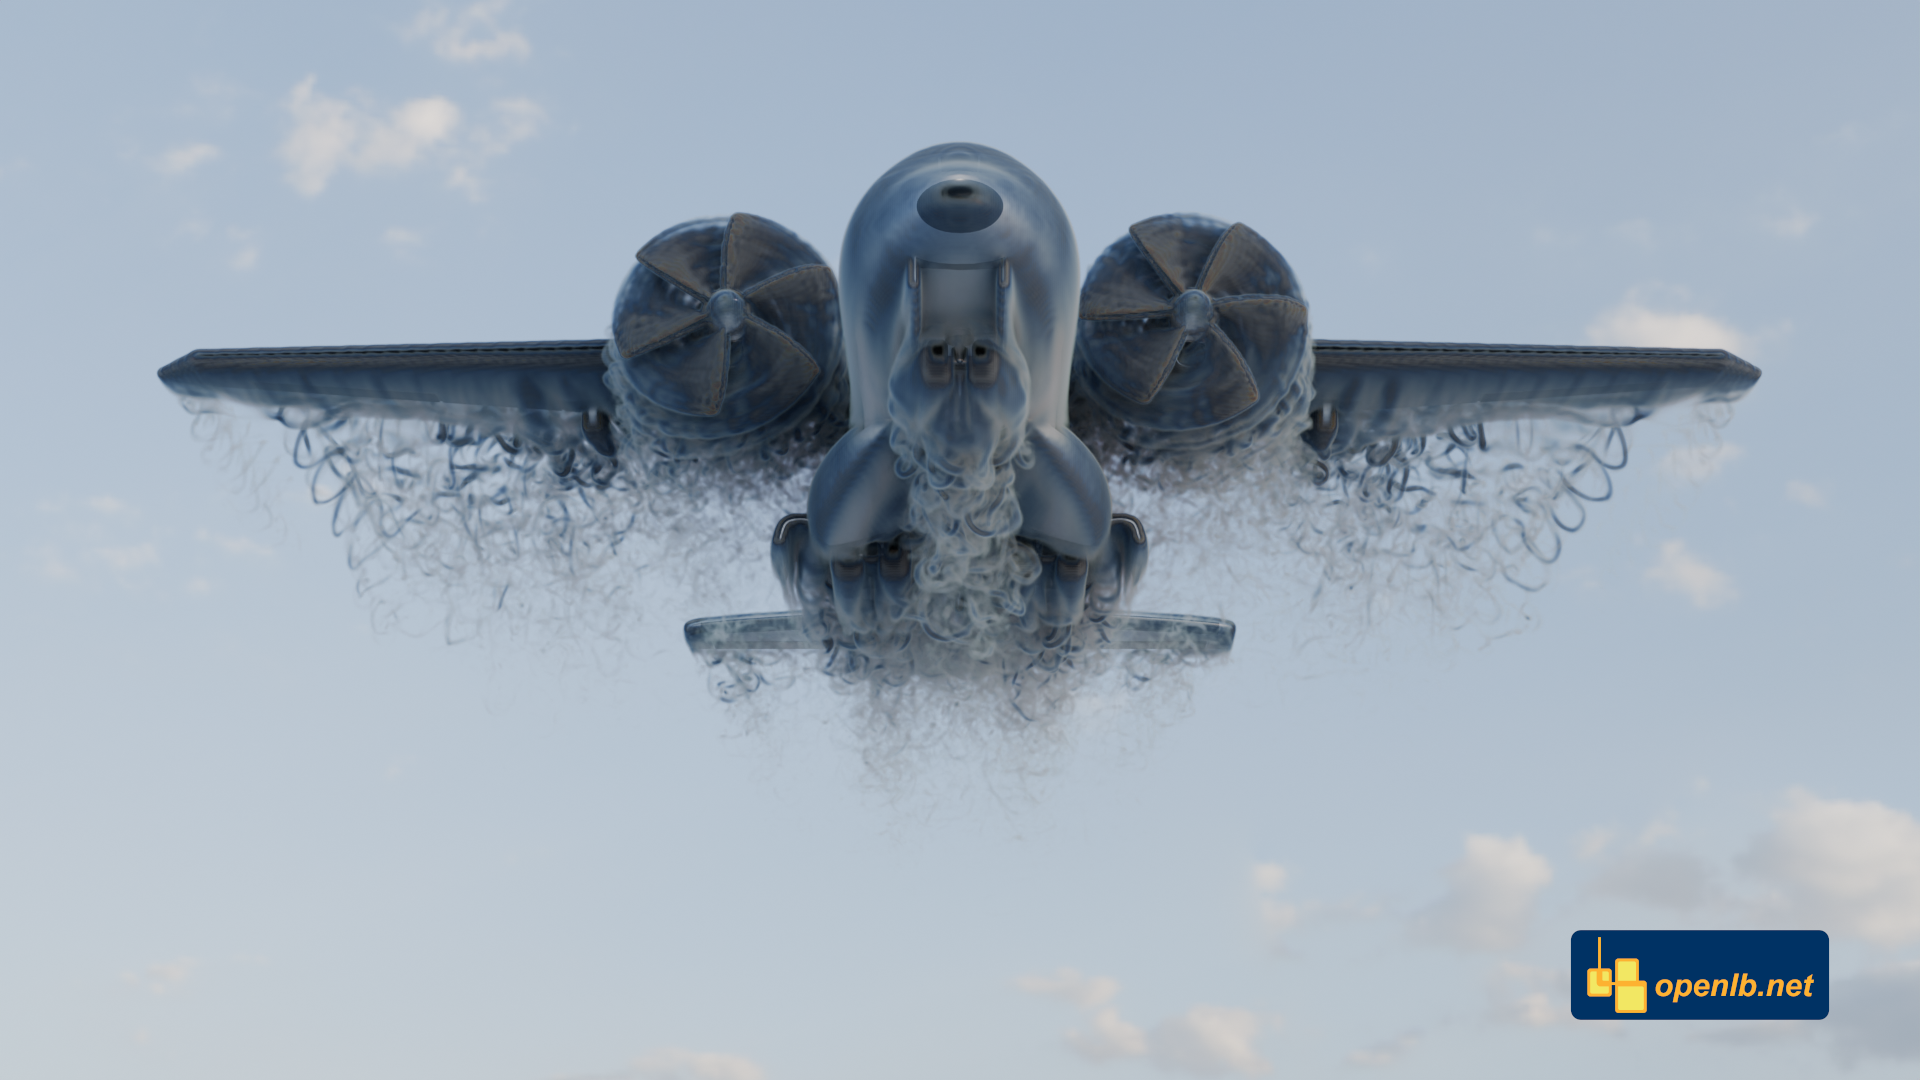
\includegraphics[width=\textwidth,angle=0,trim={0 7cm 0 0},clip]{fig/airbusBlenderPreview2-with-logo.png}
		\end{center}
	}; 
	%% Authors and Date
	\node[text width=1.0\textwidth] at ($$ (current page.south) + (0mm,+90mm) $$){
		\begin{center}
		{ \textbf{Authors:} }
      Adrian Kummerl\"{a}nder,
      Tim N.\ Bingert,
      Fedor Bukreev,
      Luiz E.\ Czelusniak,
      Davide Dapelo,
      Simon Englert,
      Christoph Gaul,
      Michael Grinschewski,
      Shota Ito,
      Julius Jeßberger,
      Florian Kaiser,
      Danial Khazaeipoul,
      Timm Kr\"{u}ger,
      Halim Kusumaatmaja,
      Jan E.\ Marquardt,
      František Prinz,
      Alice Raeli,
      Michael Rennick,
      Maximilian Schecher,
      Andreas Schneider,
      Yuji Shimojima,
      Stephan Simonis,
      Pascal Sitter,
      Philipp Spelten,
      Alexandre Tacques,
      Dennis Teutscher,
      Mingliang Zhong,
      Mathias J.\ Krause
		\end{center}
	};
	%% Logo
	\node[text width=1.0\textwidth] at ($$ (current page.south) + (0mm,+35mm) $$){
    \begin{flushright}
		
\includegraphics[width=5cm]{fig/openlb_full.png}
	\end{flushright}
	};
	\end{tikzpicture}
\end{titlepage}

\centerline{Date: \today}
\centerline{Copyright \copyright{} 2006-2008 Jonas Latt}
\centerline{Copyright \copyright{} 2008-2025 Mathias J.\ Krause}
\centerline{\href{mailto:info@openlb.net}{\nolinkurl{info@openlb.net}}}\vspace{1cm}

Permission is granted to copy, distribute and/or modify this document
under the terms of the GNU Free Documentation License, Version 1.2
or any later version published by the Free Software Foundation;
with no Invariant Sections, no Front-Cover Texts, and no Back-Cover
Texts.  A copy of the license is included in the Section entitled ``GNU
Free Documentation License'' (Section~\ref{sec:license}).

\begin{abstract}
\OpenLB is a generic implementation of lattice Boltzmann methods (LBM) that is shared with the open source community under the terms of the GPLv2 license.
Since the first release in 2007 \cite{olb03}, the code continues to be improved and extended, resulting in sixteen major releases~\cite{olb18,olb17,olb16,olb15,olb14,olb13,olb12,olb11,olb10,olb09,olb08,olb07,olb06,olb05,olb04,olb03} overall and counting.
The \OpenLB framework is written in C++ and covers the full scope of simulations -- from pre-processing over parallel and efficient execution to post-processing of results.
It offers both the possibility of setting up new simulation cases using the existing rich collection of models and of implementing new custom models.
\OpenLB supports MPI, OpenMP, AVX(51)2 vectorization, and CUDA for parallel execution on systems ranging from low-end smartphones over multi-GPU workstations up to supercomputers.
\end{abstract}